\documentclass[10pt,aspectratio=169]{beamer}
% Packages
\usepackage{mathabx}
\usepackage{xcolor}
\usepackage{amsmath}
\usepackage{mathtools}
\usepackage{standalone}
\usepackage{mhchem}
\usepackage{textpos}
\usepackage{graphicx}
\usepackage{wrapfig}
\usepackage{booktabs}
\usepackage{textcomp}
\usepackage{makecell}
\usepackage{wasysym}

\usepackage{tikz}
\usetikzlibrary{shapes,arrows,positioning,fit}

\usepackage{pgfplots}
\pgfplotsset{compat=1.18}

\usepackage{listings}
\lstset{
basicstyle=\small\ttfamily,
columns=flexible,
breaklines=true
}

\graphicspath{{images}}

% Configure template
\setbeamertemplate{navigation symbols}{}

% Theme
\usetheme[progressbar=frametitle]{metropolis}
\setbeamertemplate{caption}[numbered]
\setbeamersize{text margin left=5mm,text margin right=5mm}

% Title page details:
\title{Scientific Computing: Molecular dynamics}
\subtitle{Problemsheet 5}
\author{Jimin Kim, Christian Nix, Noah Schlenker}
\date{19. July 2024}
\institute{Technical University of Munich}

\begin{document}

% Title page frame
    \maketitle

    \addtobeamertemplate{frametitle}{}{
        \begin{textblock*}{100mm} (.945\textwidth,-.85cm)
            
\includegraphics[scale=0.14]{../template/res/tum_logo.png}
        \end{textblock*}}

% Outline frame
    \begin{frame}{Outline}
        \tableofcontents
    \end{frame}

% Slides
    \section{Membrane}
\label{sec:membrane}

\begin{frame}
    \frametitle{Molecular abstraction}
    
    \begin{itemize}
        \item Molecule class allows future extensions to different molecules and potentials
        \item Has own intra-molecular forces using \texttt{calculateIntraMolecularForces} method
        \item Molecule class offers \texttt{generateMolecule} method to construct the molecule
    \end{itemize}

    \vspace{7pt}
    \hrule

    \begin{columns}
        \begin{column}{0.6\textwidth}
            \begin{itemize}
                \item Membrane class inherits from molecule class
                \item A membrane is generated as a cuboid cluster
                \item Introduced a unique ID attribute for particles (which is their index within the particle cluster)
                \item[] \!\!\!\!\!\!\!\!\! \textcolor{orange}{$\Rightarrow$} Allowed us to store only the molecular IDs in the neighbor maps
                \item By storing only half of the neighbors we enabled parallel force calculations by using Newton's third law (stencil)
                \item The Membrane takes care of its own forces and must only be disregarded in the other force calculations
            \end{itemize}
        \end{column}
        \begin{column}{0.4\textwidth}
            \begin{figure}
                \centering
                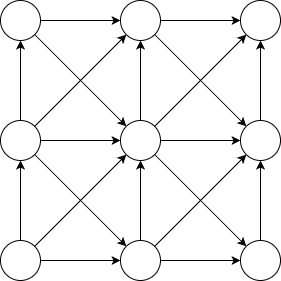
\includegraphics[width=0.6\columnwidth]{../../res/membraneNeighbor.drawio}
                \caption{Neighborhood of particles. Results in directed non-cyclic graph.}
                \label{fig:mem}
            \end{figure}
        \end{column}
    \end{columns}

    
\end{frame}
    \section{Parallelization}
\label{sec:parllel}

\begin{frame}
    \frametitle{Parallelization}

    \begin{columns}
        \begin{column}{0.5\textwidth}
            \centerline{
                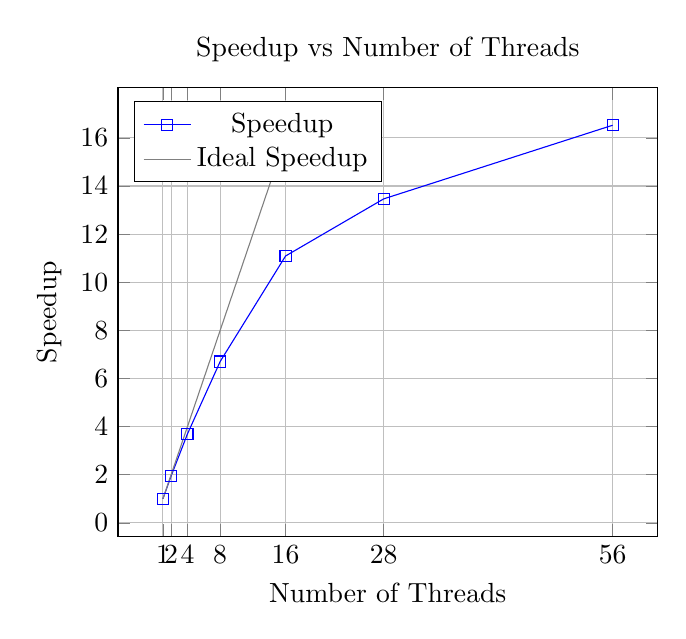
\begin{tikzpicture}
                \begin{axis}[
                    title={Speedup vs Number of Threads},
                    xlabel={Number of Threads},
                    ylabel={Speedup},
                    grid=both,
                    xtick={1, 2, 4, 8, 16, 28, 56},
                    ytick={0, 2, 4, 6, 8, 10, 12, 14, 16},
                    legend pos=north west
                ]
                \addplot[
                    color=blue,
                    mark=square,
                    ]
                    coordinates {
                    (1, 1)
                    (2, 3272 / 1680)
                    (4, 3272 / 885)
                    (8, 3272 / 488)
                    (16, 3272 / 295)
                    (28, 3272 / 243)
                    (56, 3272 / 198)
                    };

                    \addplot[
                    color=gray,
                    ]
                    coordinates {
                    (1, 1)
                    (16, 16)
                    };
                \addlegendentry{Speedup}
                \addlegendentry{Ideal Speedup}
                \end{axis}
                \end{tikzpicture}
            }
        \end{column}
            \begin{column}{0.5\textwidth}
                \begin{figure}
                    \centering
                    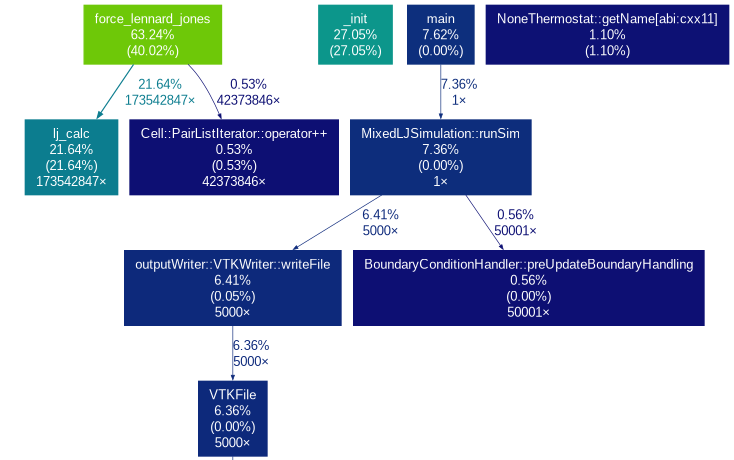
\includegraphics[width=\columnwidth]{../../res/optimized.png}
                    \caption{Visualization of runtime distributions.}
                    \label{fig:runtime}
                \end{figure}
            \end{column}
    \end{columns}


\end{frame}
    \section{Nano-Scale Flow}
\label{sec:nano}

\begin{frame}
    \frametitle{Nano-Scale flow}
    
    \begin{columns}
        \begin{column}{0.3\textwidth}
            \begin{itemize}
                \item We ran 5 simulations
                \item Base simulation did not generate directed flow
                \item After setting $\sigma = 0.8$, $\epsilon = 5.0$, and $g_{grav}=-9.81$, we obtained a nice result
            \end{itemize}

            \vspace{7pt}
            \hrule
            \vspace{7pt}

            \begin{itemize}
                \item Particles are immobilized by type
                \item Analytics are measured in multiple dimensions
                \item Python script can generate profile from vtk
            \end{itemize}
        \end{column}
        \begin{column}{.7\textwidth}
            \begin{figure}
                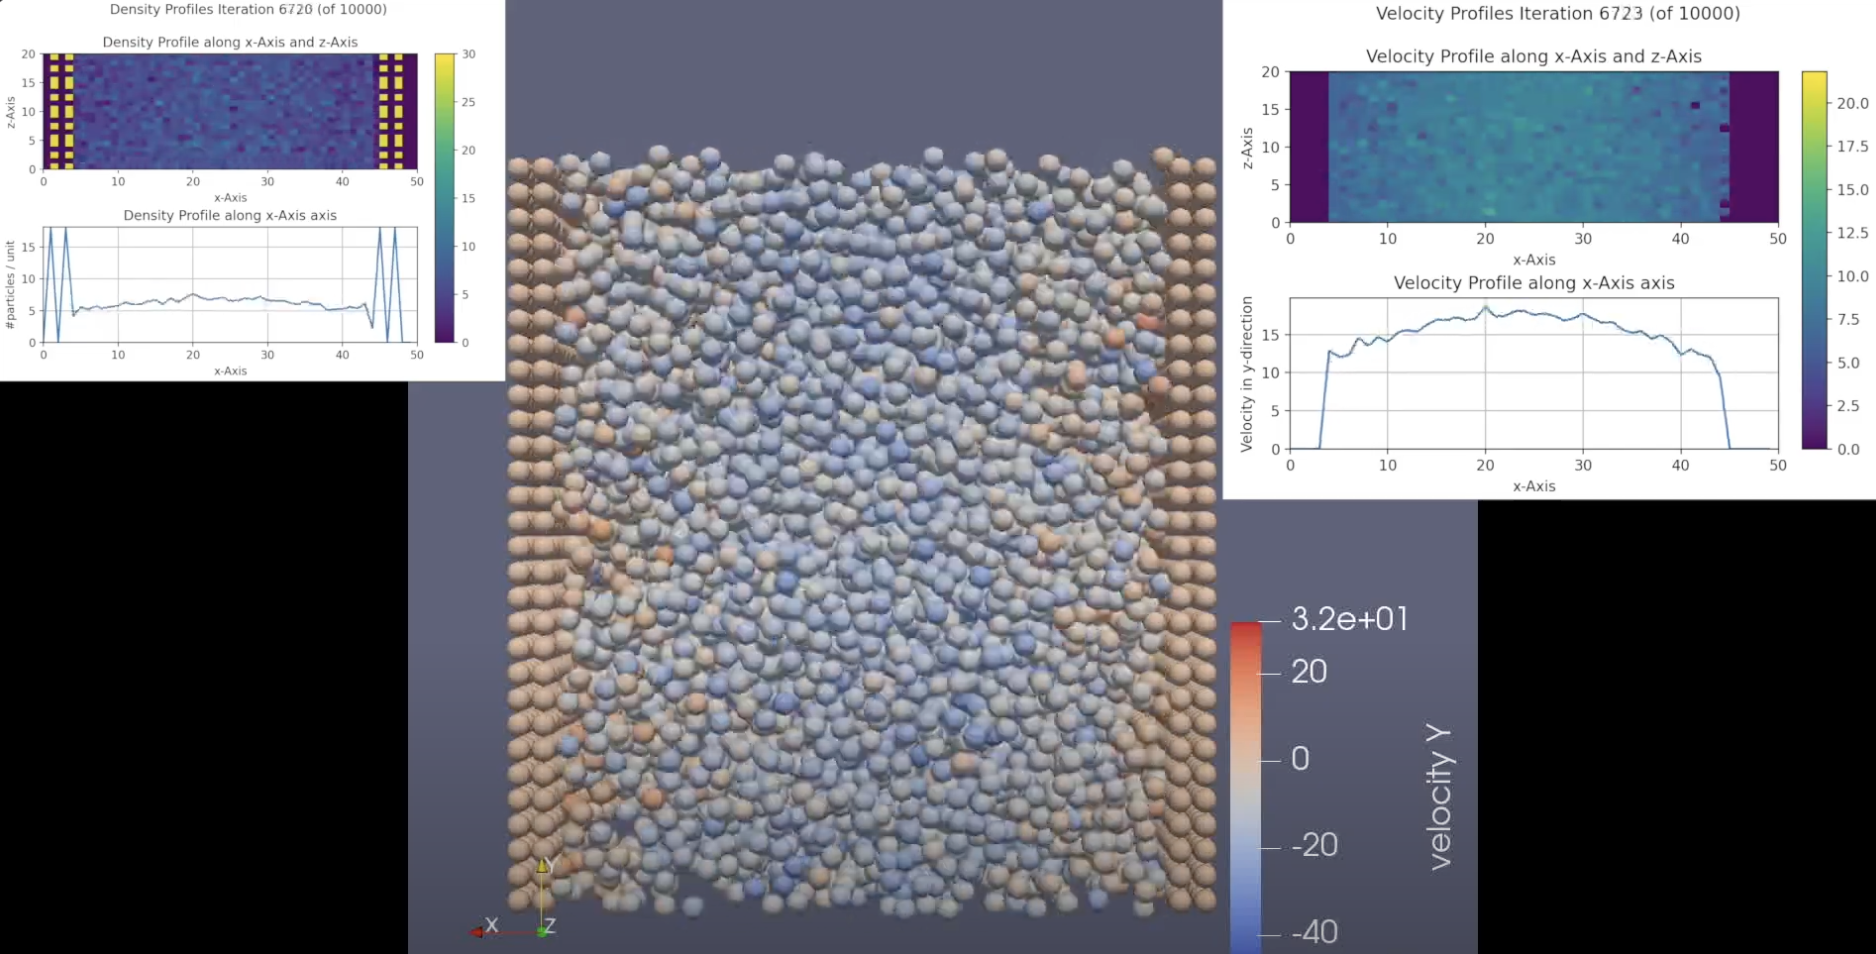
\includegraphics[width=\columnwidth]{../../res/Stronger_walls_nano_flow.png}
                \caption{Stronger wall slows particles on the borders while gravity accelerates the center.}
                \label{fig:strong-walls}
            \end{figure}
        \end{column}
    \end{columns}
    
    
\end{frame}
    
\section{Analytics}
\label{sec:analytics}

\begin{frame}
    \frametitle{Analytics}
    

\end{frame}

\end{document}